\documentclass{article}
\usepackage[margin=1in]{geometry}
\usepackage{amsmath,amsthm,amssymb}
\usepackage{bbm,enumerate,mathtools}
\usepackage{tikz,pgfplots}
\usepackage{chessboard}
\usepackage[hidelinks]{hyperref}
\usepackage{multicol} % Problem 35
\usepackage{xstring} % Difficulty command
\usetikzlibrary{shapes.geometric}

\newenvironment{question}{\begin{trivlist}\item[\textbf{Question.}]}{\end{trivlist}}
\newenvironment{note}{\begin{trivlist}\item[\textbf{Note.}]}{\end{trivlist}}
\newenvironment{references}{\begin{trivlist}\item[\textbf{References.}]}{\end{trivlist}}
\newenvironment{related}{\begin{trivlist}\item[\textbf{Related.}]\end{trivlist}\begin{enumerate}}{\end{enumerate}}

\newcommand\score[1]{
\pgfmathsetmacro\pgfxa{#1+1}
\tikzstyle{scorestars}=[
  star,
  star points=5,
  star point ratio=2.25,
  draw,
  inner sep=3pt,
  anchor=outer point 5
]
  \begin{tikzpicture}[baseline]
    \draw[opacity=0] (0,-0.5) rectangle (0,0.2); % Workaround for whitespace at the bottom.
    \foreach \i in {1,...,4} {
      \pgfmathparse{(\i<=#1?"yellow":"gray")}
      \edef\starcolor{\pgfmathresult}
      \draw (\i*4.5ex,0) node[name=star\i,scorestars,fill=\starcolor]  {};
    }
  \end{tikzpicture}
}

\newcommand{\difficulty}[1]{%
  \IfEqCase{#1}{%
      {1}{
        
\begin{tikzpicture}[scale=0.7, baseline=0.9mm]%
          \definecolor{slopegreen}{rgb}{0.0, 0.5, 0.0}%
          \fill[slopegreen] (0.5,0.5) circle (0.5);%
        \end{tikzpicture}%
      }%
      {2}{
        
\begin{tikzpicture}[scale=0.7, baseline=0.9mm]%
          \definecolor{slopeblue}{rgb}{0.0, 0.44, 1.00}
          \fill[slopeblue] (0,0) rectangle (1,1);%
        \end{tikzpicture}%
      }%
      {3}{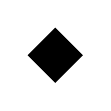
\begin{tikzpicture}[scale=0.7, baseline=0.9mm]\fill (0,0.5)--(0.5, 0)--(1,0.5)--(0.5,1)--cycle; \end{tikzpicture}}%
      {4}{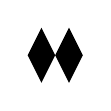
\begin{tikzpicture}[scale=0.7, baseline=0.9mm]\fill (0.25,0)--(0,0.5)--(0.25,1)--(0.5,0.5)--cycle; \fill (0.75,0)--(0.5,0.5)--(0.75,1)--(1,0.5)--cycle;\end{tikzpicture}}%
      % you can add more cases here as desired
  }[\PackageError{difficulty}{Undefined difficulty level: #1}{}]%
}%
\newcommand{\rating}[2]{\difficulty{#1}\\\score{#2}\\}


\begin{document}
\rating{2}{2}
Let $a_3(n)$ be the least $k > n$ such that $nk$ or $nk^2$ is a cube, and
let $A299117$ be the image of $a_3(n)$.
% \begin{figure}[!h]
%   \centering
  \allowdisplaybreaks
  \begin{multicols}{3}
    \noindent
    \begin{alignat*}{2}
      a_3(1)  &= 8   &&\text{ via } 1  \cdot 8     = 2^3 \\
      a_3(2)  &= 4   &&\text{ via } 2  \cdot 4     = 2^3 \\
      a_3(3)  &= 9   &&\text{ via } 3  \cdot 9     = 3^3 \\
      a_3(4)  &= 16  &&\text{ via } 4  \cdot 16    = 4^3 \\
      a_3(5)  &= 25  &&\text{ via } 5  \cdot 25    = 5^3 \\
      a_3(6)  &= 36  &&\text{ via } 6  \cdot 36    = 6^3 \\
      a_3(7)  &= 49  &&\text{ via } 7  \cdot 49    = 7^3 \\
      a_3(8)  &= 27  &&\text{ via } 8  \cdot 27    = 6^3 \\
      a_3(9)  &= 24  &&\text{ via } 9  \cdot 24    = 6^3 \\
      a_3(10) &= 80  &&\text{ via } 10 \cdot 80    = 20^3 \\
      a_3(11) &= 88  &&\text{ via } 11 \cdot 88    = 22^3 \\
      a_3(12) &= 18  &&\text{ via } 12 \cdot 18    = 6^3 \\
      a_3(13) &= 104 &&\text{ via } 13 \cdot 104^2 = 52^3 \\
      a_3(14) &= 112 &&\text{ via } 14 \cdot 112^2 = 56^3 \\
      a_3(15) &= 120 &&\text{ via } 15 \cdot 120^2 = 60^3 \\
      a_3(16) &= 32  &&\text{ via } 16 \cdot 32    = 8^3 \\
      a_3(17) &= 136 &&\text{ via } 17 \cdot 136^2 = 68^3 \\
      a_3(18) &= 96  &&\text{ via } 18 \cdot 96    = 12^3 \\
      a_3(19) &= 152 &&\text{ via } 19 \cdot 152^2 = 76^3 \\
      a_3(20) &= 50  &&\text{ via } 20 \cdot 50    = 10^3 \\
      a_3(21) &= 168 &&\text{ via } 21 \cdot 168^2 = 84^3 \\
      a_3(22) &= 176 &&\text{ via } 22 \cdot 176^2 = 88^3 \\
      a_3(23) &= 184 &&\text{ via } 23 \cdot 184^2 = 92^3 \\
      a_3(24) &= 72  &&\text{ via } 24 \cdot 72    = 12^3 \\
      a_3(25) &= 40  &&\text{ via } 25 \cdot 40    = 10^3 \\
      a_3(26) &= 208 &&\text{ via } 26 \cdot 208^2 = 104^3 \\
      a_3(27) &= 64  &&\text{ via } 27 \cdot 64    = 12^3 \\
      a_3(28) &= 98  &&\text{ via } 28 \cdot 98    = 14^3 \\
      a_3(29) &= 232 &&\text{ via } 29 \cdot 232^2 = 116^3 \\
      a_3(30) &= 240 &&\text{ via } 30 \cdot 240^2 = 120^3 \\
    \end{alignat*}
  \end{multicols}
% \end{figure}
\begin{question}
  Is there another way to characterize what integers are in $A299117$?
\end{question}

\begin{note}
  The function $a_3$ is an injection.\\
  $A299117$ contains every cube, because $a(n^3) = (n + 1)^3$.\\
  $A299117$ contains the square of every prime, because $a(p) = p^2$.
\end{note}

\begin{related}
  \item Does $A299117$ contain every square?
  \item Does $A299117$ contain any squarefree number?
  \item What about the generalization: the image of $a_\beta$ where $a_\beta(n)$
    is the least $k > n$ such that $nk$, $nk^2, \hdots, nk^{\beta-2}$, or $nk^{\beta-1}$
    is a $\beta$-th power? Prime $\beta$ is an injection---is this well behaved?
\end{related}

\begin{references}
  \item \url{https://oeis.org/A277781}
  \item \url{https://oeis.org/A299117}
\end{references}

\end{document}
